% file: 3-9-connectivity/2conn-edges-cycle.tex

\documentclass[tikz]{standalone}
\usetikzlibrary{positioning, decorations.pathmorphing}

\begin{document}
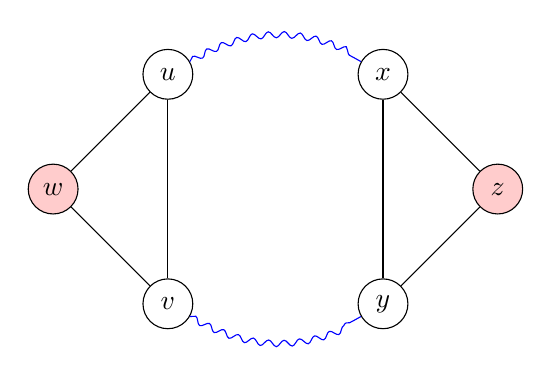
\begin{tikzpicture}[every node/.style = {draw, circle, minimum size = 18pt},
    path/.style = {-, decorate, decoration = {snake, amplitude = .4mm, segment length = 2mm, post length = 1mm}}]
  \node (w) [fill = red!20] {$w$};
  \node (z) [fill = red!20, right = 5.0cm of w] {$z$};

  \node (u) [above right = of w] {$u$};
  \node (v) [below right = of w] {$v$};

  \node (x) [above left = of z] {$x$};
  \node (y) [below left = of z] {$y$};

  \path (w) edge (u)
            edge (v)
  	(z) edge (x)
            edge (y)
  	(u) edge (v)
  	(x) edge (y)
	(u) edge[blue, bend left, path] (x)
	(v) edge[blue, bend right, path] (y);
\end{tikzpicture}
\end{document}
